\chapter{Introduction}\label{chap:introduction}
\subsection{Galaxy}
Galaxy {\footnote{\url{https://usegalaxy.eu/}}} is an open-source biological data processing and research platform. It supports numerous types of extensively used biological data formats like FASTA, FASTAQ, GFF, PDB and many more. To process these datasets, Galaxy offers tools and workflows which either transform these datasets from one type to another or manipulate them. A simple example of data processing is to merge two compatible datasets to make one. Another example can be to reverse complement a sequence of nucleotides \footnote{\url{https://usegalaxy.eu/?tool_id=MAF_Reverse_Complement_1&version=1.0.1&__identifer=zmk9dx9ivbk}}.

\begin{figure}[h]
\begin{centering}
    {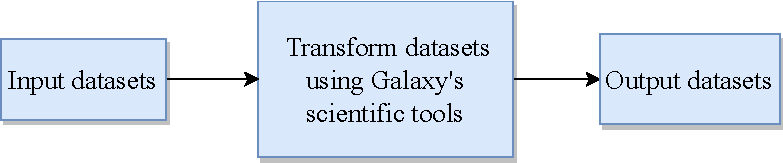
\includegraphics[scale=0.8]{figures/image_Galaxy_1.pdf}}
    \caption[Basic flow of dataset transformation]{\textbf{Basic flow of dataset transformation}: it shows the basic flow of dataset transformation using Galaxy tools and workflows}
\end{centering}
\end{figure}

A tool is a data-transforming entity which allows one or more types of datasets, transforms these datasets and produces output datasets. The tools are classified under multiple categories based on their functions. For example, the tools which manipulate text like replacing texts and selecting first lines of a dataset are grouped together under "Text Manipulation" group.

These tools form the building blocks of workflows. The workflows are data processing pipelines where a set of tools are joined one after another. The connected tools need to be compatible to each other which means the output types of one tool should be present in the input types of the next tool. A workflow can have one or more starting and ending tools.

\subsection{Galaxy tools}
A tool entails a specific function. It consumes datasets, brings about some transformations and produces output datasets which can be fed to other tools. A tool has multiple attributes which include its input and output file types, name, description, help text and so on. They carry more information about a tool. When we look at the collective information about all these attributes for multiple tools, we find that some tools have similar functionalities based on their similarities in their corresponding attributes. For example, there are tools which share similarities in their respective functions and the input and output dataset types they are glued to. For example, a tool "hicexplorer hicpca" \footnote{\url{https://usegalaxy.eu/?tool_id=toolshed.g2.bx.psu.edu/repos/bgruening/hicexplorer_hicpca/hicexplorer_hicpca/2.1.0&version=2.1.0&__identifer=5kcqmvb71gx}}  has an output type named "bigwig". Hence, if there is a tool or a set of tools which also has "bigwig" as their input and/or output type, we consider there could be some similarity between "hicexplorer hicpca" and the other tools as they do transformations on similar types of datasets. In addition, we can find similar functions of tools by analyzing their "name" and "description" attributes. Let's take an example of two tools (Figure 2):
 
\begin{figure}[h]
\begin{centering}
    {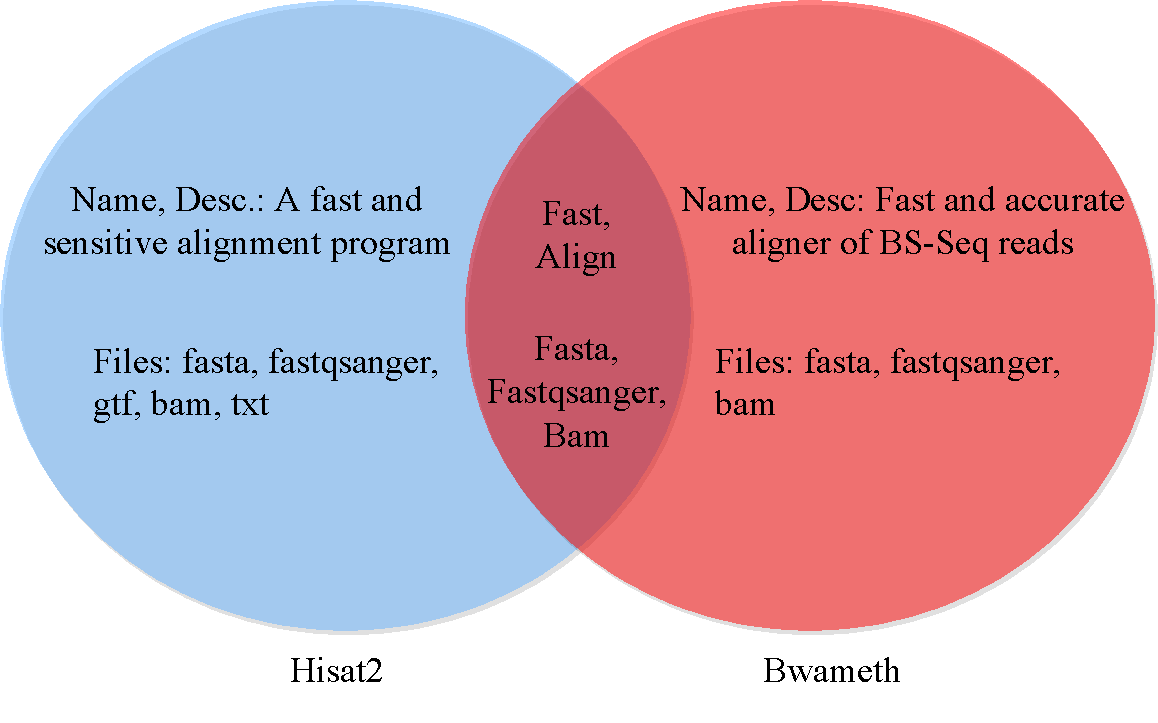
\includegraphics[scale=0.5]{figures/Venn_common_tools_info.pdf}}
    \caption[Venn diagram]{\textbf{Venn diagram}: it shows common features extracted from multiple attributes for the two tools}
\end{centering}
\end{figure}

In figure 2, we take two tools - "Linear Regression" and "Logistic Regression" and collect their respective information from their input, output file types, name and description attributes. We see that these tools share features in the venn diagram. They both do regression and few file types are also common. In the same way, if we extrapolate this venn diagram and match one tool against all other tools, we hope to find a set of tools similar in nature to the former tool. While searching for the related tools for a tool, it is possible that we end up with an empty set.

\subsection{Motivation}
From figure 2, we see that there can be tools which share characteristics. Galaxy has thousands of tools having a diverse set of functions. Moreover, new tools are keep getting added to the older set of tools. From a user's perspective, it is hard to keep knowledge about so many tools. It is important to make a user aware of the presence of new tools added. If there is a model which dispenses a clue that there is a set of say $n$ tools which are similar to a tool, it would give more options to a user for her/his data processing. 

\begin{figure}[h]
\begin{centering}
    {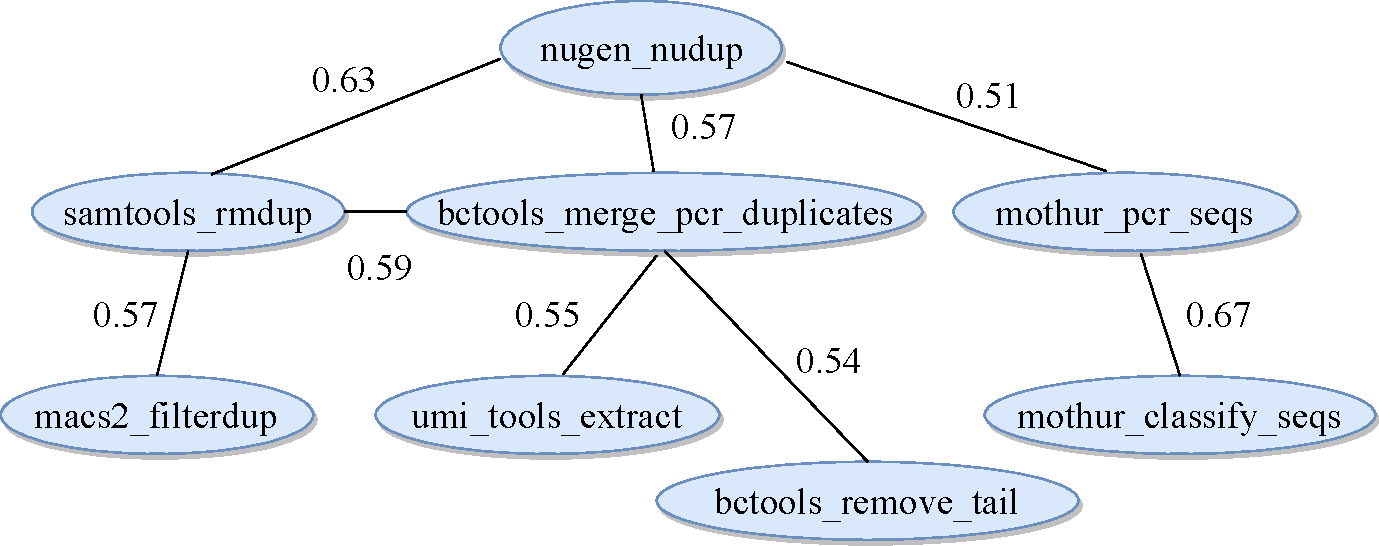
\includegraphics[scale=0.5]{figures/tools_sim_know_graph.pdf}}
    \caption[Similarity knowledge network]{\textbf{Similarity knowledge network}: it shows how the tools in the network are related. The real numbers show the relation strength}
\end{centering}
\end{figure}

To elaborate it more, let's take an example of a tool "nugen nudup" \footnote{\url{ https://toolshed.g2.bx.psu.edu/repository?repository_id=4f614394b93677e3 }}. It is used to find and remove PCR duplicates. The similar tools for it can be "samtools rmdup" and "bctools merge pcr duplicates" which work on related concepts. These similar tools would further have their respective set of similar tools thereby making a network of related entities (tools). This "knowledge network" can help a user find multiple ways to process her/his data and exhibits a exhibits "connectedness/relation" among tools. The strength of this relation may vary from being small to large. We learn a continuous representation of the relation strength. Figure 2 shows how this graph can evolve. First, we find similar tools for "nugen nudup" and connect them to their source tool specifying the similarity values as real numbers at the edges. These similar tools further have their own sets of similar tools and so on.

